%\usepackage{}
\documentclass{article}
\usepackage{setspace}
\usepackage{listings}
\usepackage{color}
\usepackage{xcolor}
\usepackage{geometry}
\usepackage{graphicx}
\usepackage{booktabs}
\usepackage{multirow}
\usepackage[normalem]{ulem}
\usepackage{tabularx}
\usepackage{hyperref}
\usepackage{enumitem}
\usepackage{indentfirst}
\usepackage{vhistory}
\geometry{a4paper,bindingoffset=0.2in,%
	left=0.75in,right=0.75in,top=0.75in,bottom=0.75in,%
	footskip=.25in}
\usepackage{natbib}
\setcitestyle{square}
\usepackage{algpseudocode}

\onehalfspacing

\newcounter{mnum}
\newcommand{\mthemnum}{M\themnum}
\newcommand{\mref}[1]{M\ref{#1}}

%opening
\title{MECHTRON 4TB6: System Design \\ LifeLine}
\author{Group 30 \\ Emily Crowe, crowee \\ Arthur Faron, farona \\ Danushka Fernando, fernad12 \\Yerin Thevarajah, thevaryn \\ Phillip Truong, truonp1}

\begin{document}

    \date{January 4, 2021}
	\maketitle
	
	\newpage
	
	\begin{versionhistory}
	    \vhEntry{0}{04/01/2021}{EC|AF|DF|YT|PT}{Document Created}
	\end{versionhistory}
	
	\newpage
    
	\tableofcontents
	\listoffigures
    \listoftables

	\newpage

    \section{Introduction}
	\subsection{Purpose}
	The purpose of LifeLine is to provide first-aiders with a device to quantitatively monitor a casualty's vital signs to assist in first aid situations.The following document will provide details of the system design of the LifeLine device. The document will serve as a record of the design variables and considerations.
    
    Decomposing a system into modules is a commonly accepted approach to development.  A module is a work assignment for a developer or development team \citep{ParnasEtAl1984}.  We advocate a decomposition
    based on the principle of information hiding \citep{Parnas1972a}.  This
    principle supports design for change, because the ``secrets'' that each module
    hides represent likely future changes.  Design for change is valuable in SC,
    where modifications are frequent, especially during initial development as the
    solution space is explored.  
    
    Our design follows the rules layed out by Parnas et al. \citep{ParnasEtAl1984}, as follows:
    \begin{itemize}
    \item System details that are likely to change independently should be the
      secrets of separate modules.
    \item Each data structure is used in only one module.
    \item Any other program that requires information stored in a module's data
      structures must obtain it by calling access programs belonging to that module.
    \end{itemize}
    
     The potential readers of this document are as follows:
    
    \begin{itemize}
    \item New project members: This document can be a guide for a new project member
      to easily understand the overall structure and quickly find the
      relevant modules they are searching for.
    \item Maintainers: The hierarchical structure of the module guide improves the
      maintainers' understanding when they need to make changes to the system. It is
      important for a maintainer to update the relevant sections of the document
      after changes have been made.
    \item Designers: Once the module guide has been written, it can be used to
      check for consistency, feasibility and flexibility. Designers can verify the
      system in various ways, such as consistency among modules, feasibility of the
      decomposition, and flexibility of the design.
    \end{itemize}
    
    \subsection{Scope}
    
    The project, named LifeLine, intends to help a first-aider monitor a casualty's vital signs to keep them stable until emergency medical services (EMS) arrives. This project also intends to assist a first-aider by retrieving vital signs quantitatively. These results can then guide the first-aider to adapt and improve their treatment plan. The device is able to record and save the vital sign data which can later be exported for more advanced analysis by medical professionals.
    \paragraph{}
    LifeLine is a product that carries out four (4) primary functions: quantitative measurement of primary vital signs through sensor readings, logging the primary vitals data, displaying the primary vitals data, and exporting the primary vitals data. The primary vital signs this project will be measuring are body temperature, blood pressure and heart rate. 
	\paragraph{}
	The device will instruct the user where to place the different sensors for each vital sign in order to measure them safely and efficiently. While these procedures are taking place, the device will present the results on a display. The first-aider can use this to further their treatment and continue monitoring the vital signs until medical assistance arrives. The product will then log the measurements and export this data into an accessible file to be used for medical records and for further examination by medical professionals. 
    
	\section{Variables}
	
	\subsection{Monitored Variables}
	    \begin{longtable}{|l|p{0.4\linewidth}|l|p{0.2\linewidth}|}
	    \caption{Monitored variables}
        \hline
        \textbf{Name} & \textbf{Description} & \textbf {Type} & \textbf{Units} \\
        \endhead
        \hline
m\_BT\_casualty  & Pre-processed Body Temperature measurement   recorded by IR temperature sensor                                               & Digital & degrees Celsius      \\ \hline
m\_BP\_casualty  & Pre-processed Blood Pressure measurement recorded   by MAX32664 sensor                                                       & Digital & mmHg    \\ \hline
m\_HR\_casualty  & Pre-processed Heart Rate measurement recorded by MAX32264   sensor                                                           & Digital & BPM     \\ \hline

\end{longtable}

	\subsection{Controlled Variables}
	
	  \begin{longtable}{|l|p{0.4\linewidth}|p{0.2\linewidth}|l|}
	  \caption{Controlled Variables}
        \hline
        \textbf{Name} & \textbf{Description} & \textbf {Type} & \textbf{Units} \\
        \endhead
        \hline
        c\_screenDisplay   & Displays data and menus requested by the user on the LCD screen of the device. & Various. Depends on what is being displayed. & N/A \\ \hline
        \end{longtable}

	\section{Constants}
	\begin{longtable}{|l|p{0.4\linewidth}|p{0.2\linewidth}|p{0.2\linewidth}|}
	  \caption{Constant Variables}
        \hline
    \textbf{Variable name}  & \textbf{Description} & \textbf{Type of Variable} & \textbf{Units}          \\ 
    \endhead
    \hline
    k\_BT\_min & Acceptable minimum body temperature & Constant & Degree Celsius \\ \hline
    k\_BT\_max & Acceptable maximum body temperature & Constant & Degree Celsius \\ \hline
    k\_BP\_min & Acceptable minimum blood pressure & Constant & mmHg \\ \hline
    k\_BP\_max & Acceptable maximum blood pressure & Constant & mmHg \\ \hline
    k\_HR\_min & Acceptable minimum heart rate & Constant         & BPM            \\ \hline
    k\_HR\_max & Acceptable maximum heart rate & Constant         & BPM            \\ \hline
    \end{longtable}
    \newpage
    \section {Module Components}
    \begin{description}
    Module \ref{BT_M}: Body Temperature Measurement\\
    Module \ref{BP_M}: Blood Pressure Measurement \\
    Module \ref{HR_M}: Heart Rate Measurement \\
    Module \ref{casualty_mod}: Casualty Module Interface Specification (MIS) \\
    Module \ref{BT_DP}: Body Temperature Data Processing \\
    Module \ref{BP_DP}: Blood Pressure Data Processing \\
    Module \ref{HR_DP}: Heart Rate Data Processing \\
    Module \ref{DS}: Data Storage \\
    Module \ref{DE}: Data Exporting \\
    Module \ref{UI_O_F}: User Interface- On/Off \\
    Module \ref{UI_DV}: User Interface- Display Values \\
    Module \ref{UI_DSS}: User Interface- Display System Status \\
    Module \ref{UI_SS}: User Interface- System Settings \\
    
        \begin{figure}[!htb]
    	\centering
    	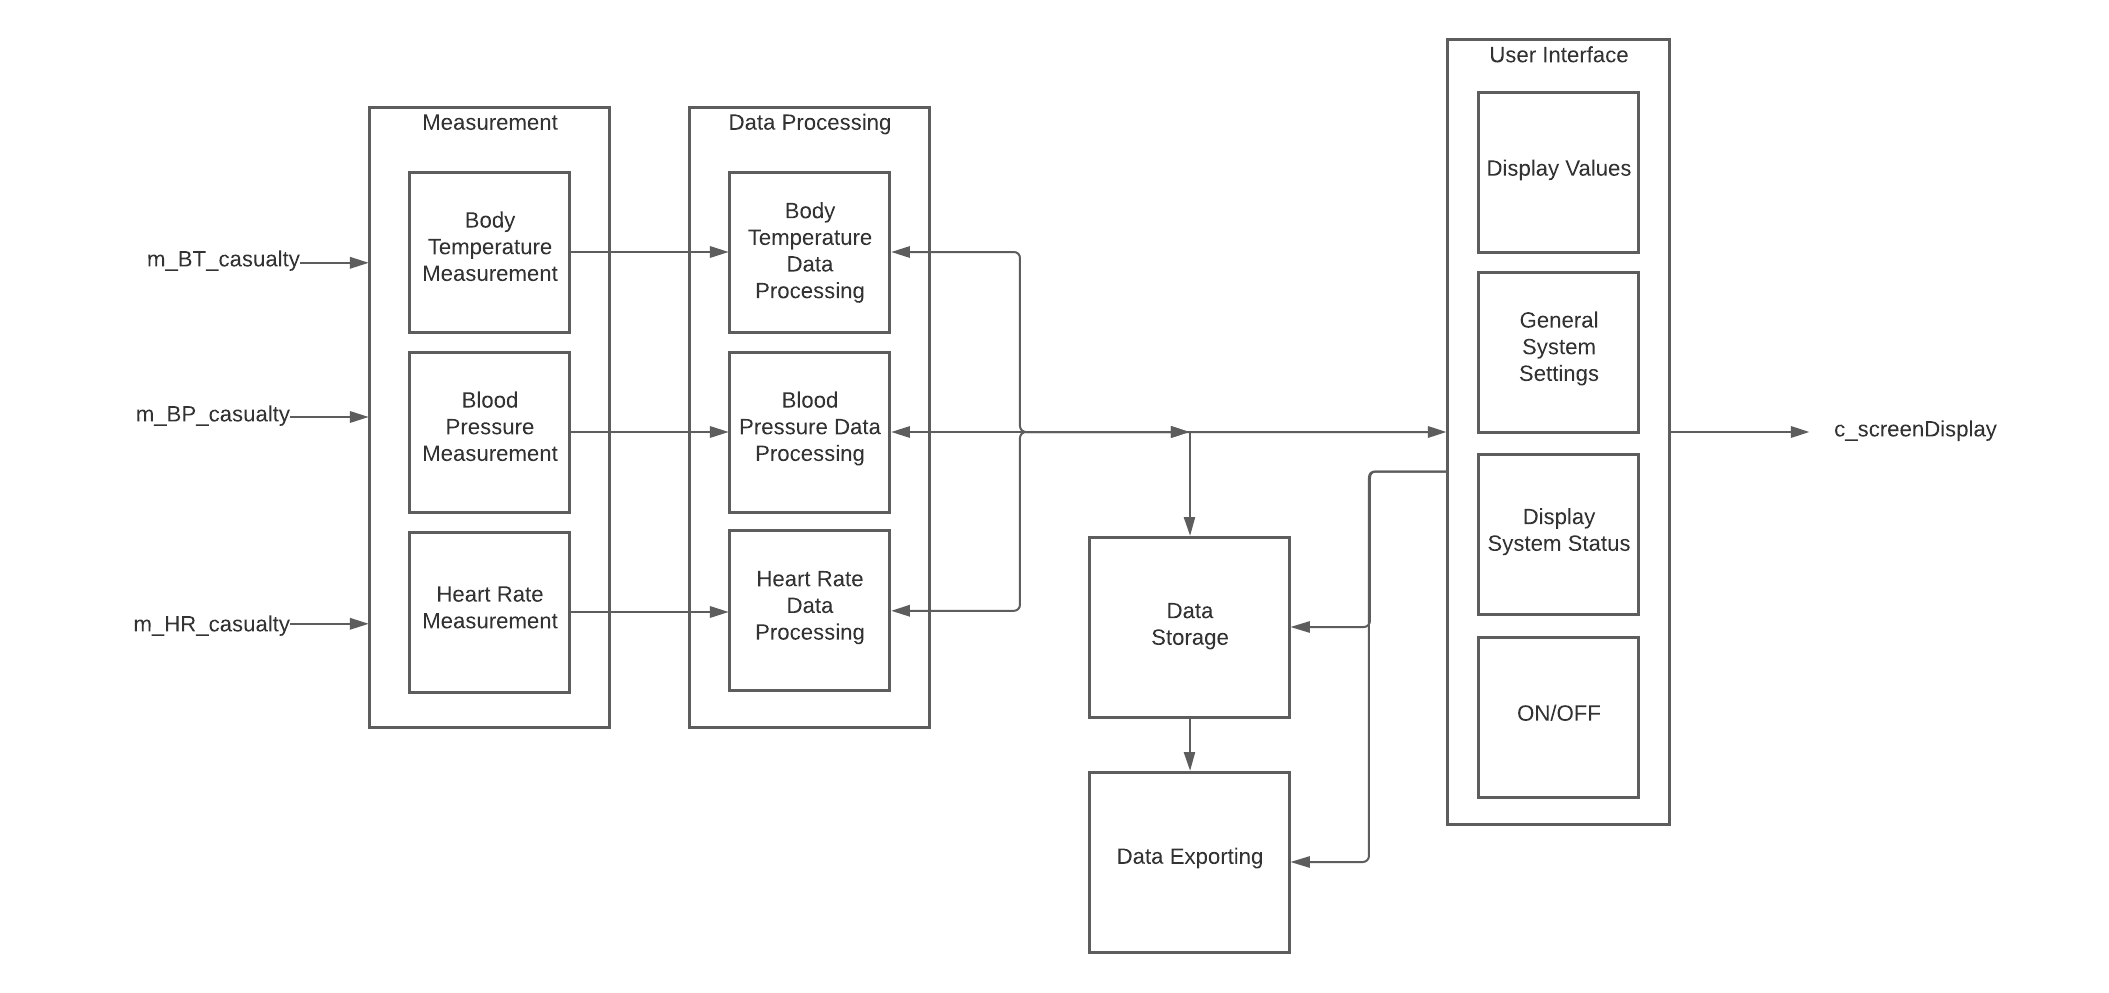
\includegraphics[width=1\linewidth]{module overview rev2.png}
    	\caption{Module overview}{Outlines the modules including in the LifeLine system and how they interact with each other.}
    \end{figure}
    
    \begin{figure}[!htb]
    	\centering
    	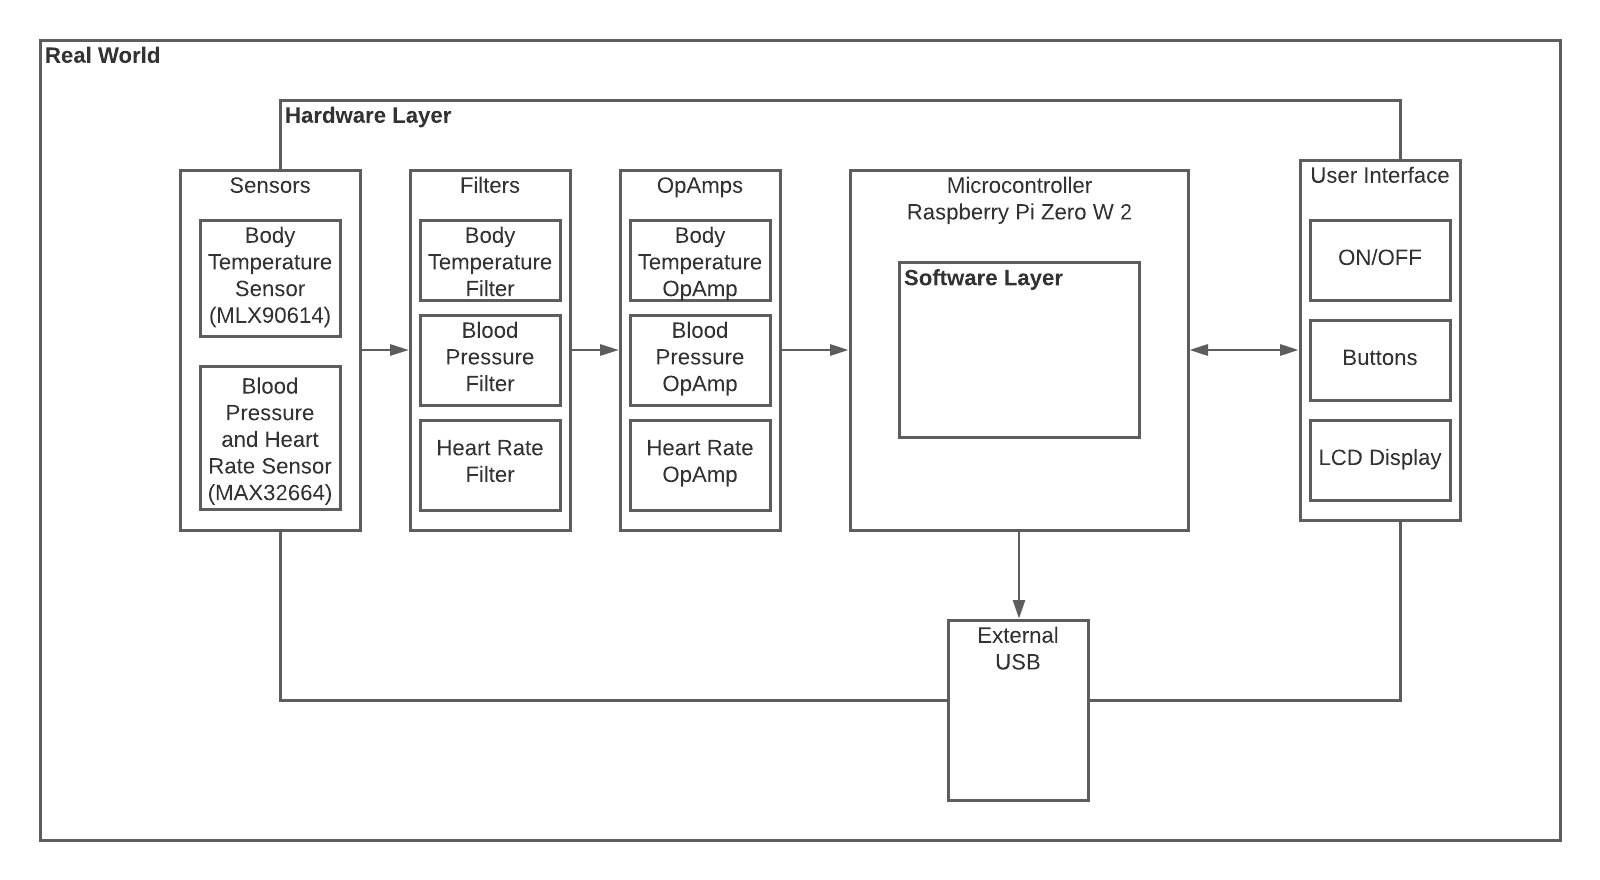
\includegraphics[width=1\linewidth]{component overview rev2.png}
    	\caption{Hardware overview}{Outlines the main hardware components used in the LifeLine device.}
    \end{figure}
    

    \newpage
    \subsection {Body Temperature Measurement} 
    \item [\refstepcounter{mnum} \mthemnum \label{BT_M}:] Body Temperature Measurement\\
    
    %Body Temperature Diagram
    \begin{figure}[!htb]
    	\centering
    	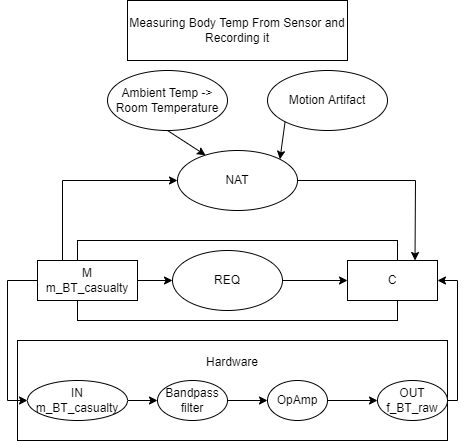
\includegraphics[width=0.5\linewidth]{mccharts-BodyTempModule.drawio.png}
    	\caption{Body Temperature Measurement Mapping}
    	{NAT: Ambient temperature can affect the performance of the body temperature component since the MLX90614 IR thermometer operates best at room temperature. Motion artifact caused by any movements of the casualty has the potential to impact the body temperature measurement.}
    \end{figure}    
        
        \subsubsection{Services}
        The body temperature measurement module uses the MLX90614 IR thermometer (sensor) to measure the body temperature of the casualty.
        \subsubsection{Secrets}
        The body temperature measurement module handles raw data input from the body temperature sensor and passes it to the 'Body Temperature Data Processing' (M\ref{BT_DP}). The body temperature module performs analog filtering of the input signal from the sensor. This raw temperature value is sent to the 'Body Temperature Data Processing' (M\ref{BT_DP}) and 'Data Storage' (M\ref{DS}) modules.
        
        \subsubsection{Inputs and Outputs}
        Sensor is placed on the casualty's body for body temperature measurement.
            \begin{longtable}{|l|p{0.4\linewidth}|l|p{0.2\linewidth}|}
            \caption{Body Temperature Measurement Input Variables}
            \hline
            \textbf{Input Variable} & \textbf{Description} & \textbf {Data Type} & \textbf{From Module} \\
            \endhead
            \hline
            m\_BT\_casualty & Casualty's temperature as received by MLX90614 IR thermometer & Digital & N/A \\
            
            \hline
            \end{longtable}
            \begin{longtable}{|l|p{0.4\linewidth}|l|p{0.2\linewidth}|}
            \caption{Body Temperature Measurement Output Variables}
            \hline
            \textbf{Output Variable} & \textbf{Description} & \textbf {Data Type} & \textbf{To Module} \\
            \endhead
            \hline
            f\_BT\_raw & Raw body temperature data processed by bandpass filter and operational amplifier & Double & Body Temperature Data Processing (M\ref{BT_DP}), Data Storage (M\ref{DS}) \\
            \hline
            \end{longtable}
        \subsubsection{Software Components}
        None.
        \subsubsection{Hardware Components}
        \begin{itemize}
            \item MLX90614 IR thermometer
            \item Bandpass filter
            \item Operational amplifier
        \end{itemize}
        \subsubsection{Timing Constraints}
        There must be no more than 1 second to receive measurement from sensor to display (NFR4 in System Requirements).  The MLX90614 IR thermometer takes 0.25 seconds to acquire data from start-up \citep{melexis}.
    \newpage 
    
    \subsection{Blood Pressure Measurement} 
    \item [\refstepcounter{mnum} \mthemnum \label{BP_M}:] Blood Pressure Measurement
    %Blood Pressure Diagram
    \begin{figure}[!htb]
    	\centering
    	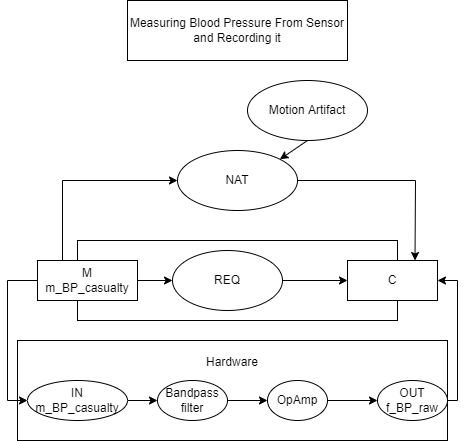
\includegraphics[width=0.5\linewidth]{mccharts-BloodPressureModule.drawio.png}
    	\caption{Blood Pressure Measurement Mapping}
    	{NAT: Motion artifact caused by any movements of the casualty has the potential to impact the blood pressure measurement.}
    \end{figure} 
        
        \subsubsection{Services}
        The blood pressure measurement module uses the Pulse Express Pulse-Ox \& Heart Rate Sensor with MAX32664 (sensor) to measure the blood pressure trending of the casualty.
        \subsubsection{Secrets}
        The blood pressure measurement module handles raw data input from the blood pressure sensor and passes it to 'Blood Pressure Data Processing' (M\ref{BP_DP}). The blood pressure measurement module performs analog filtering of the input signal from the sensor. This raw temperature value is sent to the 'Blood Pressure Data Processing' (M\ref{BP_DP}) and 'Data Storage' (M\ref{DS}) modules.
        \subsubsection{Input}
            \begin{longtable}{|l|p{0.4\linewidth}|l|p{0.2\linewidth}|}
            \caption{Blood Pressure Measurement Input Variables}
            \hline
            \textbf{Input Variable} & \textbf{Description} & \textbf {Data Type} & \textbf{From Module} \\
            \endhead
            \hline
            m\_BP\_casualty & Casualty's blood pressure as received by MAX32664 & Analog & N/A \\
            \hline
            \end{longtable}
        \newpage
        \subsubsection{Output}
            \begin{longtable}{|l|p{0.25\linewidth}|l|p{0.25\linewidth}|}
            \caption{Blood Pressure Measurement Output Variables}
            \hline
            \textbf{Output Variable} & \textbf{Description} & \textbf {Data Type} & \textbf{To Module} \\
            \endhead
            \hline
            f\_BP\_raw & Raw blood pressure data processed by bandpass filter and operational amplifier & Double & Blood Pressure Data Processing (M\ref{BP_DP}), Data Storage (M\ref{DS}) \\
            \hline
            \end{longtable}
        \subsubsection{Software Components}
        None.
        \subsubsection{Hardware Components}
        \begin{itemize}
            \item MAX32664 Optical Biometric Hub
            \item bandpass filter
            \item operational amplifier
        \end{itemize}
     
        \subsubsection{Timing Constraints}
        There must be no more than 1 second to receive measurement from sensor to display (NFR4 in System Requirements).  The MAX32664 has a clock speed of 96MHz \citep{false}.
    \newpage
    
    
    \subsection{Heart Rate Measurement} 
    \item [\refstepcounter{mnum} \mthemnum \label{HR_M}:] Heart Rate Measurement
    %Heart Rate Diagram
    \begin{figure}[!htb]
    	\centering
    	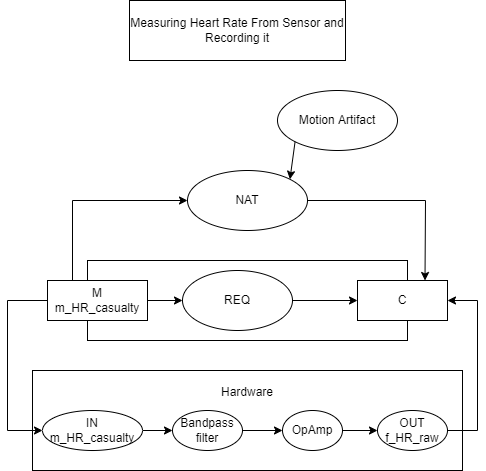
\includegraphics[width=0.5\linewidth]{mccharts-HeartRateModule.drawio.png}
    	\caption{Heart Rate Measurement Mapping}
    	{NAT: Motion artifact caused by any movements of the casualty has the potential to impact the heart rate measurement.}
    \end{figure}
        \subsubsection{Services}
        The heart rate measurement module uses the Pulse Express Pulse-Ox \& Heart Rate Sensor with MAX32664 (sensor) to measure the heart rate of the casualty.
        \subsubsection{Secrets}
        The heart rate measurement module handles raw data input from the heart sensor and passes it to 'Heart Rate Data Processing' (M\ref{HR_DP}). The heart rate measurement module performs analog filtering of the input signal from the sensor. This raw temperature value is sent to the 'Heart Rate Data Processing' (M\ref{HR_DP}) and 'Data Storage' (M\ref{DS}).
    
        \subsubsection{Input}
            \begin{longtable}{|l|p{0.4\linewidth}|l|p{0.2\linewidth}|}
            \caption{Heart Rate Measurement Input Variables}
            \hline
            \textbf{Input Variable} & \textbf{Description} & \textbf {Data Type} & \textbf{From Module} \\
            \endhead
            \hline
            m\_HR\_casualty & Casualty's heart rate as received by MAX32664 & Analog & N/A \\
            \hline
            \end{longtable}
        \newpage
        \subsubsection{Output}
            \begin{longtable}{|l|p{0.4\linewidth}|l|p{0.2\linewidth}|}
            \caption{Heart Rate Measurement Output Variables}
            \hline
            \textbf{Output Variable} & \textbf{Description} & \textbf {Data Type} & \textbf{To Module} \\
            \endhead
            \hline
            f\_HR\_raw &  Raw heart rate data processed by bandpass filter and operational amplifier & Double & Blood Pressure Data Processing (M\ref{HR_DP}), Data Storage (M\ref{DS})\\
            \hline
            \end{longtable}
        \subsubsection{Software Components}
        None.
        \subsubsection{Hardware Components}
        \begin{itemize}
            \item MAX32664 Optical Biometric Hub
            \item bandpass filter
            \item operational amplifier
        \end{itemize}
        \subsubsection{Timing Constraints}
        There must be no more than 1 second to receive measurement from sensor to display (NFR4 in System Requirements).  The MAX32664 has a clock speed of 96MHz \citep{false}.
    \newpage
    
    \subsection{Casualty Data Component}
    \item [\refstepcounter{mnum} \mthemnum \label{casualty_mod}:] Casualty Data Component
    \section* {Casualty Module Interface Specifications}

        \subsection*{Module}
        
        CasualtyT
        
        \subsection* {Uses}
        
        None
        
        \subsection* {Syntax}
        
        \subsubsection* {Exported Constants}
        
        None
        
        \subsubsection* {Exported Types}
        
        None
        
        \subsubsection* {Exported Access Programs}
        
        \begin{tabular}{| l | l | l | p{5cm} |}
          \hline
          \textbf{Routine name} & \textbf{In} & \textbf{Out} & \textbf{Exceptions}\\
          \hline
          new\_CasualtyT & & CasualtyT & \\
          \hline
          getRawBodyTemp &  & f\_BT\_raw: double & \\
          \hline
          getRawBloodPres & & f\_BP\_raw: double& \\
          \hline
          getRawHeartRate & & f\_HR\_raw: double & \\
          \hline
          getBodyTemp & & f\_BT\_proc: double & measureAgain\\
          \hline
          getBloodPres & & f\_BP\_proc: double & measureAgain\\
          \hline
          getHeartRate & & f\_HR\_proc: double  & measureAgain\\
          \hline
          setRawBodyTemp & f\_BT\_raw: double   & & \\
          \hline
          setRawBloodPres & f\_BP\_raw: double & & \\
          \hline
          setRawHeartRate & f\_HR\_raw: double & & \\
          \hline
          setBodyTemp & f\_BT\_raw: double & & measureAgain\\
          \hline
          setBloodPres & f\_BP\_raw: double & & measureAgain\\
          \hline
          setHeartRate & f\_HR\_raw: double & & measureAgain\\
          \hline
          
          
        \end{tabular}
        
        \subsection* {Semantics}
        
        \subsubsection* {State Variables}
        
        $\mathit{casualtyID}$: int \\
        $\mathit{f\_BT\_raw}$: double \\
        $\mathit{f\_BP\_raw}$: double \\
        $\mathit{f\_HR\_raw}$: double \\
        $\mathit{f\_BT\_proc}$: double\\
        $\mathit{f\_BP\_proc}$: double \\
        $\mathit{f\_HR\_proc}$: double \\
        $\mathit{f\_BT\_sensorOK}$: bool\\
        $\mathit{f\_BP\_sensorOK}$: bool \\
        $\mathit{f\_HR\_sensorOK}$: bool \\
        
        \subsubsection* {State Invariant}
        
        None
        
        \subsubsection* {Assumptions}
        
        The state variables will be set before they are used.
        
        \subsubsection* {Access Routine Semantics}
        
        \noindent new CasualtyT():
        \begin{itemize}
        \item transition: $\mathit{casualtyID}$ := generateID()
        \item output: $out := \mathit{self}$
        \item exception: none
        \end{itemize}
        
        \noindent getRawBodyTemp():
        \begin{itemize}
        \item output: $out := \mathit{f\_BT\_raw}$
        \item exception: none
        \end{itemize}
        
        \noindent getRawBloodPres():
        \begin{itemize}
        \item output: $out := \mathit{f\_BP\_raw}$
        \item exception: none
        \end{itemize}
        
        s\noindent getRawHeartRate( ):
        \begin{itemize}
        \item output: $out := \mathit{f\_HR\_raw}$
        \item exception: none
        \end{itemize}
        
        \noindent getBodyTemp():
        \begin{itemize}
        \item output: $out := \mathit{f\_BT\_proc}$
        \item exception: measureAgain()
        \end{itemize}
        
        \noindent getBloodPres():
        \begin{itemize}
        \item output: $out := \mathit{f\_BP\_proc}$
        \item exception: measureAgain()
        \end{itemize}
        
        \noindent getHeartRate():
        \begin{itemize}
        \item output: $out := \mathit{f\_HR\_proc}$
        \item exception: measureAgain()
        \end{itemize}
        
        \noindent setRawBodyTemp(\mathit{f\_BT\_raw}):
        \begin{itemize}
        
        \item exception: none
        \end{itemize}
        
        \noindent setRawBloodPres(\mathit{f\_BP\_raw}):
        \begin{itemize}
        \item exception: none
        \end{itemize}
        
        \noindent setRawHeartRate(\mathit{f\_HR\_raw}):
        \begin{itemize}
        \item exception: none
        \end{itemize}
        
        \noindent setBodyTemp(\mathit{f\_BT\_raw}):
        \begin{itemize}
        \item transition: \\
        \begin{algorithmic}
        \If{checkInRange(smoothData({f\_BT\_raw}, min, max)} 
            \State 
            f\_BT\_proc := smoothData({f\_BT\_raw})
            \State 
            f\_BT\_sensorOK := TRUE
        \Else
            \State 
            f\_BT\_sensorOK := FALSE
            \State 
            measureAgain()
        \EndIf 
        \end{algorithmic}
        \item exception: measureAgain()
        
        \end{itemize}
        
        \noindent setBloodPres(\mathit{f\_BP\_raw}):
        \begin{itemize}
        \item transition: \\
        \begin{algorithmic}
        \If{checkInRange(smoothData({f\_BP\_raw}, min, max)} 
            \State 
            f\_BP\_proc := smoothData({f\_BP\_raw})
            \State 
            f\_BP\_sensorOK := TRUE
        \Else
            \State 
            f\_BP\_sensorOK := FALSE
            \State 
            measureAgain()
        \EndIf 
        \end{algorithmic}
        \item exception: measureAgain()
        \end{itemize}
        
        \noindent setHeartRate(\mathit{f\_HR\_raw}):
        \begin{itemize}
        \item transition: \\
        \begin{algorithmic}
        \If{checkInRange(smoothData({f\_HR\_raw}, min, max)} 
            \State 
            f\_HR\_proc := smoothData({f\_HR\_raw})
            \State 
            f\_Hr\_sensorOK := TRUE
        \Else
            \State 
            f\_HR\_sensorOK := FALSE
            \State 
            measureAgain()
        \EndIf 
        \end{algorithmic}
        \item exception: measureAgain()
        \end{itemize}
        
        \subsubsection* {Local Functions}
        smoothData: rawData \rightarrow processedData\\
        smoothData(rawData)
        
        checkInRange:
        checkInRange(processedData, min, max)
        \begin{algorithmic}
        \If{smoothData({f\_BP\_raw}, min, max) $>$ min && smoothData({f\_BP\_raw}, min, max) $<$ min)}
            \State 
            return TRUE
        \Else
            \State 
            return FALSE
        \EndIf 
        \end{algorithmic}
        
        generateID: \rightarrow int
        generateID()
        
        measureAgain: \rightarrow string
        measureAgain(): print("Please Measure Again")
        
        \newpage
    
    \subsection{Body Temperature Data Processing} 
    \item [\refstepcounter{mnum} \mthemnum \label{BT_DP}:] Body Temperature Data Processing
    
     \begin{figure}[!htb]
    	\centering
    	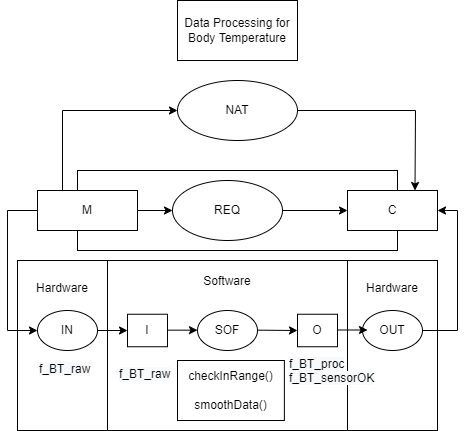
\includegraphics[width=0.5\linewidth]{mccharts-BTDataProc.drawio.png}
    	\caption{Body Temperature Data Processing Mapping}
    \end{figure}
    
    
        \subsubsection{Service}
        The body temperature data processing module reduces noise and smooths the body temperature data.  The body temperature data processing module additionally determines whether the readings are within an acceptable range.
        
        \subsubsection{Secrets}
        The body temperature data processing module handles output of the  'Body Temperature Measurement' (M\ref{BT_M}) module.  Once smoothed, it is passed to the 'Data Storage' (M\ref{DS}) module.  Additionally, the smoothed data is checked against a constant range of acceptable body temperatures and the result is stored in variable f\_BT\_sensorOK.  This variable is also passed to the 'Data Storage' (M\ref{DS}) module.
        
        \subsubsection{Input}
            \begin{longtable}{|l|p{0.4\linewidth}|l|p{0.2\linewidth}|}
            \caption{Body Temperature Data Processing Input Variables}
            \hline
            \textbf{Input Variable} & \textbf{Description} & \textbf {Data Type} & \textbf{From Module} \\
            \endhead
            \hline
            f\_BT\_raw & Raw body temperature data processed by bandpass filter and operational amplifier & Double & Body Temperature Measurement (M\ref{BT_M})\\
            \hline
            \end{longtable}
        \newpage
        \subsubsection{Output}
            \begin{longtable}{|l|p{0.4\linewidth}|l|p{0.2\linewidth}|}
            \caption{Body Temperature Data Processing Output Variables}
            \hline
            \textbf{Output Variable} & \textbf{Description} & \textbf {Data Type} & \textbf{To Module} \\
            \endhead
            \hline
            f\_BT\_proc & Processed body temperature data after digital smoothing & Double & Data Storage (M\ref{DS})\\
            \hline
            f\_BT\_sensorOK & Body temperature sensor status indicator.  True if body temperature is in acceptable range.  False if out of range. & Boolean & Data Storage (M\ref{DS})\\
            \hline
            \end{longtable}
        \subsubsection{Software Components}
                Refer to: M\ref{casualty_mod} - Casualty Software Module

                \begin{longtable}{|l|p{0.2\linewidth}|l|p{0.4\linewidth}|}
                \caption{Body Temperature Data Processing Software Components}
                \hline
                \textbf{Function} & \textbf{Parameters} & \textbf {Returns} & \textbf{Description} \\
                \endhead
                \hline
                smoothData()   & f\_BT\_raw & f\_BT\_proc & Removes noise and smooths data \\
                \hline
                checkInRange()   & f\_BT\_proc, k\_BT\_min, k\_BT\_max & f\_BT\_sensorOK & Determines whether the processed data is in range \\
                \hline
                \end{longtable}
        \subsubsection{Hardware Components}
            \begin{itemize}
            \item Raspberry Pi Zero W 2
            \end{itemize}
        \subsubsection{Timing Constraints}
        There must be no more than 1 second to receive measurement from sensor to display (NFR4 in System Requirements).
    \newpage

    \subsection{Blood Pressure Data Processing}
    \item [\refstepcounter{mnum} \mthemnum \label{BP_DP}:] Blood Pressure Data Processing
    
    \begin{figure}[!htb]
    	\centering
    	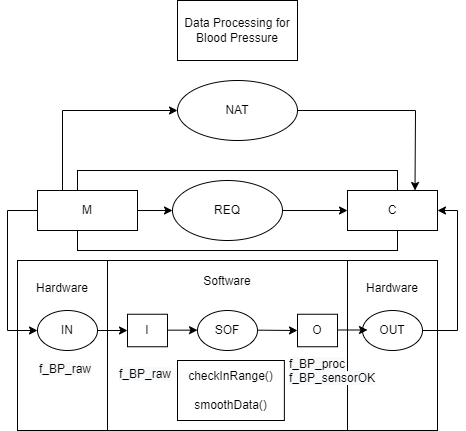
\includegraphics[width=0.5\linewidth]{mccharts-BPDataProc.drawio.png}
    	\caption{Blood Pressure Data Processing Mapping}
    \end{figure}
    
        \subsubsection{Service}
        The blood pressure data processing module reduces noise and smooths the blood pressure data. The blood pressure data processing module additionally determines whether the blood pressure readings are within an acceptable range.
        
        \subsubsection{Secrets}
        The blood pressure data processing module handles output of the 'Blood Pressure Measurement' (M\ref{BP_M}) module.  Once smoothed, it is passed to the 'Data Storage' (M\ref{DS}) module.  Additionally, the smoothed data is checked against a constant range of acceptable blood pressure measurements and the result is stored in variable f\_BP\_sensorOK.  This variable is also passed to the 'Data Storage' (M\ref{DS}) module.
        
        \subsubsection{Input}
            \begin{longtable}{|l|p{0.4\linewidth}|l|p{0.2\linewidth}|}
            \caption{Blood Pressure Data Processing Input Variables}
            \hline
            \textbf{Input Variable} & \textbf{Description} & \textbf {Data Type} & \textbf{From Module} \\
            \endhead
            \hline
            f\_BP\_raw & Raw blood pressure data processed by bandpass filter and operational amplifier & Double & Blood Pressure Measurement (M\ref{BP_M}) \\
            \hline
            \end{longtable}
        \newpage
        \subsubsection{Output}
            \begin{longtable}{|l|p{0.4\linewidth}|l|p{0.2\linewidth}|}
            \caption{Blood Pressure Data Processing Output Variables}
            \hline
            \textbf{Output Variable} & \textbf{Description} & \textbf {Data Type} & \textbf{To Module} \\
            \endhead
            \hline
            f\_BP\_proc & Processed blood pressure data after digital smoothing & Double & Data Storage (M\ref{DS}) \\
            \hline
            f\_BP\_sensorOK & Blood pressure sensor status indicator.  True if blood pressure is in acceptable range.  False if out of range. & Boolean & Data Storage (M\ref{DS}) \\
            \hline
            \end{longtable}
        \subsubsection{Software Components}
        Refer to: M\ref{casualty_mod} - Casualty Software Module
                \begin{longtable}{|l|p{0.2\linewidth}|l|p{0.4\linewidth}|}
                \caption{Blood Pressure Data Processing Software Components}
                \hline
                \textbf{Function} & \textbf{Parameters} & \textbf {Returns} & \textbf{Description} \\
                \endhead
                \hline
                smoothData()   & f\_BP\_raw & f\_BP\_proc & Removes noise and smooths data \\
                \hline
                checkInRange() & f\_BP\_proc, k\_BP\_min, k\_BP\_max & f\_BP\_sensorOK & Determines whether processed data is in range \\
                \hline
                \end{longtable}
            \noindent
        \subsubsection{Hardware Components}
            \begin{itemize}
            \item Raspberry Pi Zero W 2
            \end{itemize}
        \subsubsection{Timing Constraints}
        There must be no more than 1 second to receive measurement from sensor to display (NFR4 in System Requirements).
    \newpage

    \subsection{Heart Rate Data Processing}
    \item [\refstepcounter{mnum} \mthemnum \label{HR_DP}:] Heart Rate Data Processing
    
    \begin{figure}[!htb]
    	\centering
    	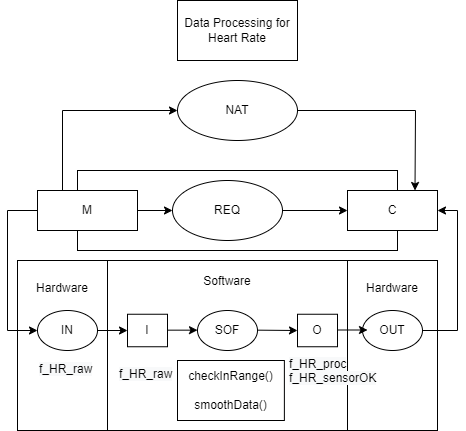
\includegraphics[width=0.5\linewidth]{mccharts-HRDataProc.drawio.png}
    	\caption{Heart Rate Data Processing Mapping}
    \end{figure}
    
        \subsubsection{Service}
        Heart rate data processing module reduces noise and smooths the heart rate data.  The heart rate data processing module additionally determines whether the heart rate readings are within an acceptable range.
        
        \subsubsection{Secrets}
        The heart rate data processing module handles output of the 'Heart Rate Measurement' (M\ref{HR_M}) module.  Once smoothed, it is passed to the 'Data Storage' (M\ref{DS}) module.  Additionally, the smoothed data is checked against a constant range of acceptable blood pressure measurements and the result is stored in variable f\_BP\_sensorOK.  This variable is also passed to the 'Data Storage' (M\ref{DS}) module.
        
        \subsubsection{Input}
            \begin{longtable}{|l|p{0.4\linewidth}|l|p{0.2\linewidth}|}
            \caption{Heart Rate Data Processing Input Variables}
            \hline
            \textbf{Input Variable} & \textbf{Description} & \textbf {Data Type} & \textbf{From Module} \\
            \endhead
            \hline
            f\_HR\_raw & Raw heart rate data processed by bandpass filter and operational amplifier & Double & Heart Rate Measurement (M\ref{HR_M})\\
            \hline
            \end{longtable}
        \newpage
        \subsubsection{Output}
            \begin{longtable}{|l|p{0.4\linewidth}|l|p{0.2\linewidth}|}
            \caption{Heart Rate Data Processing Output Variables}
            \hline
            \textbf{Output Variable} & \textbf{Description} & \textbf {Data Type} & \textbf{To Module} \\
            \endhead
            \hline
            f\_HR\_proc & Processed heart rate data after digital smoothing & Double & Data Storage (M\ref{DS}) \\
            \hline
            f\_HR\_sensorOK & Heart rate sensor status indicator.  True if heart rate is within acceptable range.  False if out of range. & Boolean &  Data Storage (M\ref{DS})\\
            \hline
            \end{longtable}
        \subsubsection{Software Components}
        Refer to: M\ref{casualty_mod} - Casualty Software Module
                \begin{longtable}{|l|p{0.2\linewidth}|l|p{0.4\linewidth}|}
                \caption{Heart Rate Data Processing Software Components}
                \hline
                \textbf{Function} & \textbf{Parameters} & \textbf {Returns} & \textbf{Description} \\
                \endhead
                \hline
                smoothData()   & f\_HR\_raw & f\_HR\_proc & Removes noise and smooths data \\
                \hline
                checkInRange() & f\_HR\_proc, k\_HR\_min, k\_HR\_max & f\_HR\_sensorOK & Determines whether processed data is in range \\
                \hline
                \end{longtable}
            \noindent
        \subsubsection{Hardware Components}
            \begin{itemize}
            \item Raspberry Pi Zero W 2
            \end{itemize}
        \subsubsection{Timing Constraints}
        There must be no more than 1 second to receive measurement from sensor to display (NFR4 in System Requirements).
    \newpage
    
    \subsection{Data Storage}
    \item [\refstepcounter{mnum} \mthemnum \label{DS}:] Data Storage
    \begin{figure}[!htb]
    	\centering
    	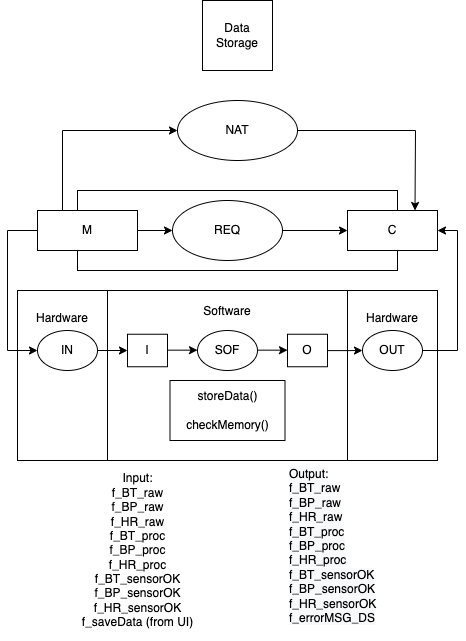
\includegraphics[width=0.5\linewidth]{mccharts-DataStorage.drawio.png}
    	\caption{Data Storage Mapping}
    \end{figure}
        \subsubsection{Services}
        Logs raw and processed sensor data as it is being collected and saves it to a patient profile. This data can later be exported to an external drive through the 'Data Exporting' (M\ref{BT_M}) module. 
        The data storage module stores both the processed and unprocessed data.  Additionally, it has the ability to separate the data saved for different patients.  If the data isn't exported, it will be deleted on a power cycle.   
        \subsubsection{Secrets}
        This module handles raw and processed data from the sensors. It detects any errors in the processed sensor data and sends a binary true/false value to the 'User Interface - Display System Status' (M\ref{UI_DSS}) module. Additionally, it saves the user's confirmation when prompted to either save or delete data from the local device. 
        \newpage
        \subsubsection{Input}
            \begin{longtable}{|l|p{0.4\linewidth}|l|p{0.2\linewidth}|}
            \caption{Data Storage Input Variables}
            \hline
            \textbf{Input Variable} & \textbf{Description} & \textbf {Data Type} & \textbf{From Module} \\
            \endhead
            \hline
            f\_BT\_raw   & Measured body temperature reading & Double & Body Temperature Measurement (M\ref{BT_M})\\
            \hline
            f\_BP\_raw   & Measured blood pressure reading & Double & Blood Pressure Measurement (M\ref{BP_M}) \\
            \hline
            f\_HR\_raw   & Measured heart rate reading & Double & Heart Rate Measurement (M\ref{HR_M})\\
            \hline
            f\_BT\_proc   & Processed body temperature reading & Double & Body Temperature Data Processing (M\ref{BT_DP})\\
            \hline
            f\_BP\_proc   & Processed blood pressure reading & Double & Blood Pressure Data Processing (M\ref{BP_DP})\\
            \hline
            f\_HR\_proc   & Processed heart rate reading & Double & Heart Rate Data Processing (M\ref{HR_DP})\\
            \hline
            f\_BT\_sensorOK   & Body temperature sensor status & Boolean & Body Temperature Data Processing (M\ref{BT_DP})\\
            \hline
            f\_BP\_sensorOK   & Blood pressure sensor status & Boolean & Blood Pressure Data Processing (M\ref{BP_DP})\\
            \hline
            f\_HR\_sensorOK   & Heart rate sensor status & Boolean & Heart Rate Data Processing (M\ref{HR_DP})\\
            \hline
            f\_saveData   & Saves user's choice to save or delete collected data & Boolean & UI-ON/OFF (M\ref{UI_O_F})\\
            \hline
            \end{longtable}
        
        \newpage
        \subsubsection{Output}
            \begin{longtable}{|l|p{0.4\linewidth}|l|p{0.2\linewidth}|}
            \caption{Data Storage Output Variables}
            \hline
            \textbf{Output Variable} & \textbf{Description} & \textbf {Data Type} & \textbf{To Module} \\
            \endhead
            \hline
            f\_BT\_raw   & Measured body temperature reading & Double & Data Export (M\ref{DE}) \\
            \hline
            f\_BP\_raw   & Measured blood pressure reading & Double & Data Export (M\ref{DE}) \\
            \hline
            f\_HR\_raw   & Measured heart rate reading & Double & Data Export (M\ref{DE}) \\
            \hline
            f\_BT\_proc   & Processed body temperature reading & Double & Data Export (M\ref{DE}), User Interface \\
            \hline
            f\_BP\_proc   & Processed blood pressure reading & Double & Data Export (M\ref{DE}), User Interface \\
            \hline
            f\_HR\_proc   & Processed heart rate reading & Double & Data Export (M\ref{DE}), User Interface \\
            \hline
            f\_BT\_sensorOK   & Body temperature sensor status & Boolean & Data Export (M\ref{DE}), User Interface \\
            \hline
            f\_BP\_sensorOK   & Blood pressure sensor status & Boolean & Data Export (M\ref{DE}), User Interface \\
            \hline
            f\_HR\_sensorOK   & Heart rate sensor status & Boolean & Data Export (M\ref{DE}), User Interface \\
            \hline
            f\_errorMSG\_DS   & Sends thrown error messages in Data Storage module to the UI Display Status module  & String & Data Export (M\ref{DE}), UI Display System Status (M\ref{UI_DSS})\\
            \hline
            \end{longtable}
        \subsubsection{Software Components}
            \noindent
            Uses: Refer to: M\ref{casualty_mod} - Casualty Software Module
                \begin{longtable}{|l|l|p{0.2\linewidth}|p{0.4\linewidth}|}
                \caption{Data Storage Software Components}
                \hline
                \textbf{Function} & \textbf{Parameters} & \textbf {Returns} & \textbf{Description} \\
                \endhead
                \hline
                storeData() & f\_saveData & N/A
                & If f\_saveData == true then data collected from sensors is saved locally on device. Otherwise data is deleted.  \\
                \hline
                checkMemory() & N/A & f\_errorMSG\_DS & Monitors the data storage module and returns errors if any are found \\
                \hline
                \end{longtable}
        \subsubsection{Hardware Components}
            \begin{itemize}
            \item Raspberry Pi Zero W 2
            \item SD card
            \end{itemize}
        \subsubsection{Timing Constraints}
        N/A
    \newpage

    \subsection{Data Exporting}
    \item [\refstepcounter{mnum} \mthemnum \label{DE}:] Data Exporting
    \begin{figure}[!htb]
    	\centering
    	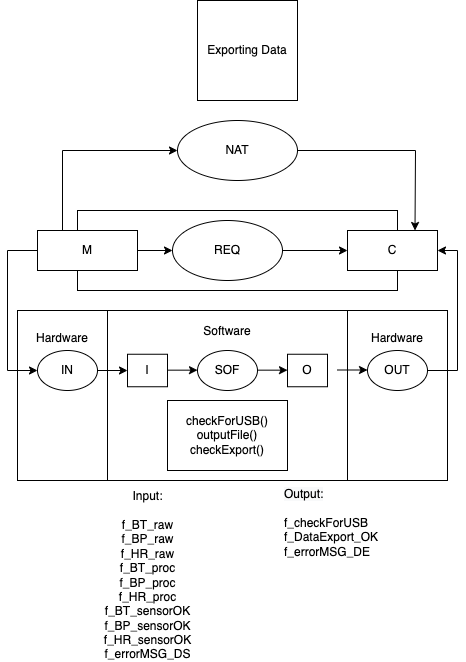
\includegraphics[width=0.5\linewidth]{mccharts-DataExport.drawio.png}
    	\caption{Data Export Mapping}
    \end{figure}
        \subsubsection{Services}
        Exports selected saved vital sign measurement data to external drive. The user can choose to export raw data, processed data, or both. 
        \subsubsection{Secrets}
         If the user chooses to export the data, the 'Data Export' (M\ref{DE}) module first checks if a USB drive has been inserted in the device. Additionally, it checks in background to see if the exporting process is carried out successfully. If it has not, it throws an error message to be displayed in the 'User Interface - Display System Status' (M\ref{UI_DSS}) module.  
        \subsubsection{Input}
            
            \begin{longtable}{|l|p{0.4\linewidth}|l|p{0.2\linewidth}|}
            \caption{Data Exporting Input Variables}
            \hline
            \textbf{Input Variable} & \textbf{Description} & \textbf {Data Type} & \textbf{From Module} \\
            \endhead
            \hline
            f\_BT\_raw   & Measured body temperature reading & Double & Data Storage (M\ref{DS}) \\
            \hline
            f\_BP\_raw   & Measured blood pressure reading & Double & Data Storage (M\ref{DS}) \\
            \hline
            f\_HR\_raw   & Measured heart rate reading & Double & Data Storage (M\ref{DS}) \\
            \hline
            f\_BT\_proc   & Processed body temperature reading & Double & Data Storage (M\ref{DS}) \\
            \hline
            f\_BP\_proc   & Processed blood pressure reading & Double & Data Storage (M\ref{DS}) \\
            \hline
            f\_HR\_proc   & Processed heart rate reading & Double & Data Storage (M\ref{DS}) \\
            \hline
            f\_BT\_sensorOK   & Body temperature sensor status & Boolean & Data Storage (M\ref{DS}) \\
            \hline
            f\_BP\_sensorOK   & Blood pressure sensor status & Boolean & Data Storage (M\ref{DS}) \\
            \hline
            f\_HR\_sensorOK   & Heart rate sensor status & Boolean & Data Storage (M\ref{DS}) \\
            \hline
            f\_errorMSG\_DS   & Consists of thrown error messages in Data Storage module  & String & Data Storage (M\ref{DS}) \\
            \hline
            \end{longtable}
        \subsubsection{Output}
            
            \begin{longtable}{|l|p{0.4\linewidth}|l|p{0.2\linewidth}|}
            \caption{Data Exporting Output Variables}
            \hline
            \textbf{Output Variable} & \textbf{Description} & \textbf {Data Type} & \textbf{To Module} \\
            \endhead
            \hline
             f\_CheckUSB   & Detects if an external drive (USB) has been inserted into the device  & Boolean & UI- Display System Status (M\ref{UI_DSS})\\ \hline
            f\_DataExport\_OK   & Detects if the export process was carried out successfully & Boolean & Data Exporting (M\ref{DE})\\ \hline
            f\_errorMSG\_DE & Sends thrown error messages in the Data Export module  & String & UI-Display System Status (M\ref{UI_DSS})\\
            \hline
            \end{longtable}
        \newpage
        \subsubsection{Software Components}
                \begin{longtable}{|p{0.25\linewidth}|p{0.2\linewidth}|p{0.2\linewidth}|p{0.30\linewidth}|}
                \caption{Data Exporting Software Components}
                \hline
                \textbf{Function} & \textbf{Parameters} & \textbf {Returns} & \textbf{Description} \\
                \endhead
                \hline
                checkforUSB()  & N/A  & f\_CheckUSB &  Check to see if a USB has been inserted in the device\\
                \hline
                outputFile()  & N/A & patientRAW.txt, patientPROC.txt & Output files to be stored in the USB Drive \\
                \hline
                checkExport()  & N/A & f\_DataExport\_OK & Ff an export issue has been detected, generate an error message and store it in f\_errorMSG\_DE \\
                \hline
                \end{longtable}
            \noindent
        \subsubsection{Hardware Components}
            \begin{itemize}
            \item Raspberry Pi Zero W 2
            \item USB drive
            \end{itemize}
    \newpage
    
    \subsection{User Interface - ON/OFF}
    \item [\refstepcounter{mnum} \mthemnum \label{UI_O_F}:] User Interface- On/Off
    \begin{figure}[!htb]
    	\centering
    	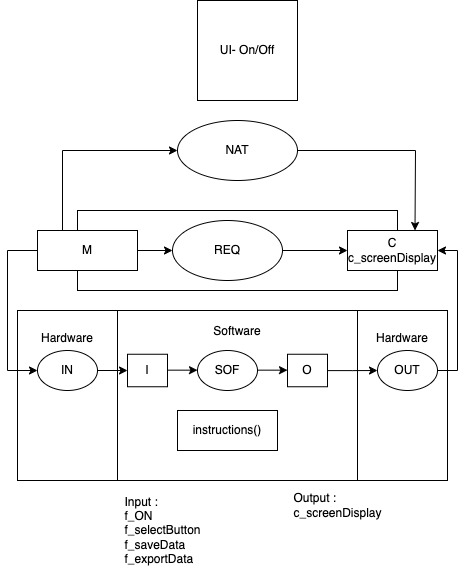
\includegraphics[width=0.5\linewidth]{mccharts-UI- ON_OFF.drawio.png}
    	\caption{User Interface - On/Off Mapping}
    \end{figure}
        \subsubsection{Services}
        A module of the user interface that is initialized by the user turning on the device to prompt placement instructions and to start measuring data.
        The turn off protocol prompts options to export and save data before turning off the device.
        \subsubsection{Secrets}
        When user turns on the device it will automatically prompt instructions to the user.
        When user selects to turn off the device it will automatically prompt the user to export and/or save data before fully turning off the device.
        \begin{figure}[!htb]
    	\centering
    	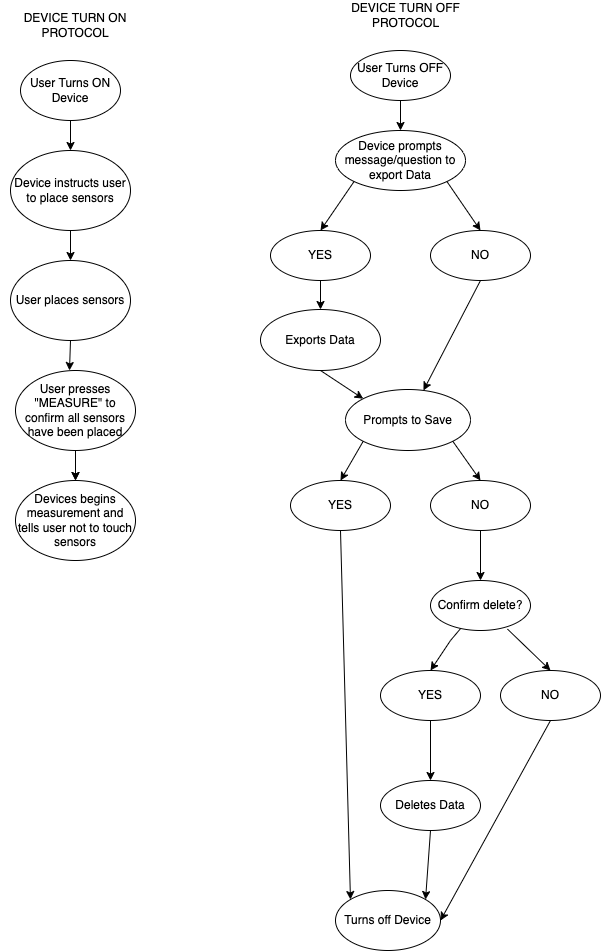
\includegraphics[width=0.65\linewidth]{flowchart-UI- ON_OFF.drawio.png}
    	\caption{Flowchart of User Interface On and Off Controls}
    \end{figure}
    \newpage
        \subsubsection{Input}
            \begin{longtable}{|l|p{0.4\linewidth}|l|p{0.2\linewidth}|}
            \caption{UI - ON/OFF Input Variables}
            \hline
            \textbf{Input Variable} & \textbf{Description} & \textbf {Data Type} & \textbf{From Module} \\
            \endhead
            \hline
            f\_ON   & State Variable if the ON button is pressed & Boolean & Set by user input \\
            \hline
            f\_startMeasure   & State Variable indicating if the 'MEASURE' button is pressed & Boolean & Set by user input \\
            \hline
            f\_saveData   & Contains user's choice to save or delete the data from the current session & Boolean & Data Storage (M\ref{DS})\\
            \hline
            f\_exportData   & Variable containing user's choice to export raw and/or processed data from the current session & Boolean & Data Export (M\ref{DE})\\
            \hline
            \end{longtable}
        \newpage
        \subsubsection{Output}
            \begin{longtable}{|l|p{0.4\linewidth}|p{0.2\linewidth}|l|}
           \caption{UI - ON/OFF Output Variables}
            \hline
            \textbf{Output Variable} & \textbf{Description} & \textbf {Data Type} & \textbf{To Module} \\
            \endhead
            \hline
            c\_screenDisplay   & Displays data and menus requested by the user on the LCD screen of the device. & Various. Depends on what is being displayed. & N/A \\
            \hline
            \end{longtable}

        \subsubsection{Software Components}
            \noindent
                \begin{longtable}{|l|p{0.35\linewidth}|l|p{0.35\linewidth}|}
                \caption{UI - ON/OFF Software Components}
                \hline
                \textbf{Function} & \textbf{Parameters} & \textbf {Returns} & \textbf{Description} \\
                \endhead
                \hline
                instructions()  & Prompted to give out instructions when user turns on the device & String & Outputs auditory and/or instructions on ideal placements of sensors for measurement\\
                \hline
                \end{longtable}
            \noindent
        \subsubsection{Hardware Components}
         \begin{itemize}
            \item Raspberry Pi Zero W 2
            \item LCD display
            \end{itemize}
    \newpage
    
    \subsection{User Interface - Display Values}
    \item [\refstepcounter{mnum} \mthemnum \label{UI_DV}:] User Interface- Display Values
    \begin{figure}[!htb]
    	\centering
    	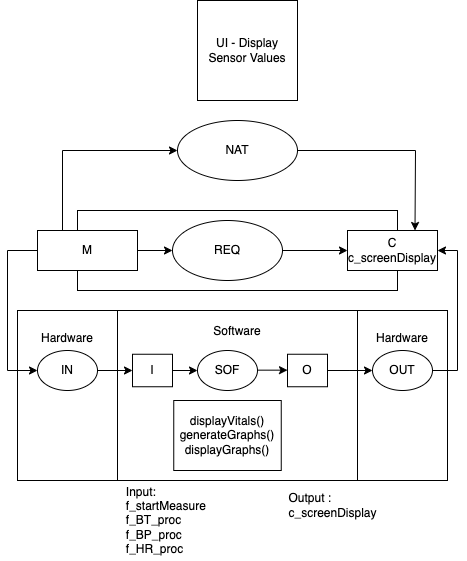
\includegraphics[width=0.5\linewidth]{DisplaySensorValues.png}
    	\caption{Mapping of User Interface - Display Values}
    \end{figure}
        \subsubsection{Services}
        A module of the user interface that displays processed vitals data and plots graphs of the data on an LCD.
        \subsubsection{Secrets}
        Graphs will be generated to be displayed on the User Interface and processed Vitals or Errors will be generated and then displayed on the User Interface
        \newpage
        \subsubsection{Input}
            \begin{longtable}{|l|p{0.4\linewidth}|l|p{0.20\linewidth}|}
            \caption{UI - Display Values Input Variables}
            \hline
            \textbf{Input Variable} & \textbf{Description} & \textbf {Data Type} & \textbf{From Module} \\
            \endhead
            \hline
            f\_startMeasure   & State Variable indicating if the 'MEASURE' button is pressed & Boolean & Set by user input \\
            \hline
            f\_BT\_proc   & Processed body temperature reading & Double & Body Temperature Data Processing (M\ref{BT_DP})\\
            \hline
            f\_BP\_proc   & Processed blood pressure reading & Double & Blood Pressure Data Processing (M\ref{BP_DP})\\
            \hline
            f\_HR\_proc   & Processed heart rate reading & Double & Heart Rate Data Processing (M\ref{HR_DP})\\
            \hline
            \end{longtable}
        \subsubsection{Output}
           \begin{longtable}{|l|p{0.4\linewidth}|p{0.2\linewidth}|l|}
           \caption{UI - Display Values Output Variables}
            \hline
            \textbf{Output Variable} & \textbf{Description} & \textbf {Data Type} & \textbf{To Module} \\
            \endhead
            \hline
            c\_screenDisplay   & Displays data and menus requested by the user on the LCD screen of the device. & Various. Depends on what is being displayed. & N/A \\
            \hline
            \end{longtable}
        \subsubsection{Software Components}
                \begin{longtable}{|l|p{0.2\linewidth}|l|p{0.4\linewidth}|}
                \caption{UI - Display Values Software Components}
                \hline
                \textbf{Function} & \textbf{Parameters} & \textbf {Returns} & \textbf{Description} \\
                \endhead
                \hline
                displayVitals()   & f\_BT\_proc f\_BP\_proc f\_HR\_proc & N/A & Displays numeric values of processed sensor readings on the LCD screen. \\
                \hline
                generateGraphs()   & f\_BT\_proc f\_BP\_proc f\_HR\_proc & Plotting data & Generates graphical representation of processed sensor readings over time.  \\
                \hline
                displayGraphs()   & Plotting data output by generateGraphs() & N/A & Displays graphs generated in generateGraphs() function on the LCD screen. \\
                \hline
                \end{longtable}
            \noindent
        \subsubsection{Hardware Components}
            \begin{itemize}
            \item Raspberry Pi Zero W 2
            \item LCD display
            \end{itemize}
    \newpage
    
    \subsection{User Interface - Display System Status}
     \begin{figure}[!htb]
    	\centering
    	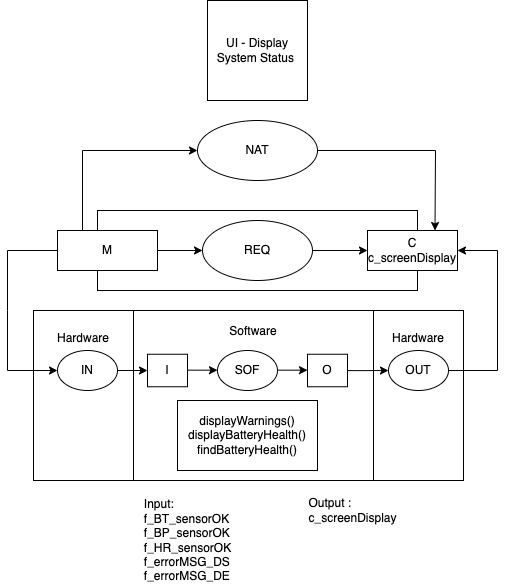
\includegraphics[width=0.5\linewidth]{mccharts-UI-DispStatus.drawio.png}
    	\caption{Mapping of User Interface - Display System Status}
    \end{figure}
    \item [\refstepcounter{mnum} \mthemnum \label{UI_DSS}:] User Interface- Display System Status
    
    
        \subsubsection{Services}
        A module of the user interface that displays system warnings and battery health of the device.
        \subsubsection{Secrets}
        Checks will be done consistently to monitor any issues with the system and battery health. If a certain issue has been returned then it will generate a warning to be displayed on the User Interface.
        \newpage
        \subsubsection{Input}
            \begin{longtable}{|l|p{0.4\linewidth}|l|p{0.2\linewidth}|}
            \caption{UI - Display System Status Input Variables}
            \hline
            \textbf{Input Variable} & \textbf{Description} & \textbf {Data Type} & \textbf{From Module} \\
            \endhead
            \hline
            f\_BT\_sensorOK   & Body temperature sensor status  & Boolean & Body Temperature Data Processing (M\ref{BT_DP})\\
            \hline
            f\_BP\_sensorOK   & Blood Pressure sensor status  & Boolean & Blood Pressure Data Processing (M\ref{BP_DP}) \\
            \hline
            f\_HR\_sensorOK   & Heart Rate sensor status & Boolean & Heart Rate Data Processing (M\ref{HR_DP}) \\
            \hline
            f\_errorMSG\_DS   & Consists of thrown error messages in Data Storage module & String & Data Storage (M\ref{DS})\\
            \hline
            f\_errorMSG\_DE   & Consists of thrown error messages in Data Export module & String & Data Export (M\ref{DE})\\
            \hline
            \end{longtable}
        \subsubsection{Output}
            \begin{longtable}{|l|p{0.4\linewidth}|p{0.2\linewidth}|l|}
           \caption{UI - Display Values Output Variables}
            \hline
            \textbf{Output Variable} & \textbf{Description} & \textbf {Data Type} & \textbf{To Module} \\
            \endhead
            \hline
            c\_screenDisplay   & Displays data and menus requested by the user on the LCD screen of the device. & Various. Depends on what is being displayed. & N/A \\
            \hline
            \end{longtable}
        \subsubsection{Software Components}
                \begin{longtable}{|l|l|l|l|}
                \caption{UI - Display System Status Software Components}
                \hline
                \textbf{Function} & \textbf{Parameters} & \textbf {Returns} & \textbf{Description} \\
                \endhead
                \hline
                displayWarnings()   & N/A & N/A  & Displays any warnings on the User Interface \\
                \hline
                displayBatteryHealth()   & N/A & N/A & Displays Battery Percentage on the User Interface \\
                \hline
                findBatteryHealth()   & N/A & N/A & Finds Battery Percentage of the Microcontroller \\
                \hline
                \end{longtable}
        \subsubsection{Hardware Components}
            \begin{itemize}
            \item Raspberry Pi Zero W 2
            \item LCD display
            \end{itemize}        
    \newpage
    
    \subsection{User Interface - System Settings}
    \item [\refstepcounter{mnum} \mthemnum \label{UI_SS}:] User Interface- System Settings
    
    \begin{figure}[!htb]
    	\centering
    	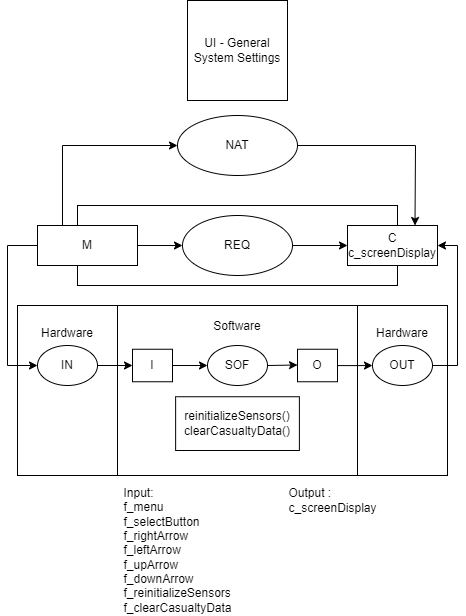
\includegraphics[width=0.5\linewidth]{mccharts-Copy of UI - SystemSettings.drawio.png}
    	\caption{Mapping of User Interface - System Settings}
    \end{figure}
    
        \subsubsection{Services}
        A module of the user interface that prompts options for re-initialization of data processing modules and options for deletion of saved casualty data.
        \subsubsection{Secrets}
        Re calibrating sensors, and resetting data processing algorithms and setting processed data to be zero and recalculating them.
        \subsubsection{Input}
            \begin{longtable}{|l|p{0.4\linewidth}|l|p{0.2\linewidth}|}
            \caption{UI - System Settings Input Variables}
            \hline
            \textbf{Input Variable} & \textbf{Description} & \textbf {Data Type} & \textbf{From Module} \\
            \endhead
            \hline
            f\_menu   & Indicates if the Menu has been selected by the user & Boolean & Set by user input \\
            \hline
            f\_selectButton   & Press button that is currently selected in Menu & Boolean & Set by user input \\
            \hline
            f\_rightArrow   & Navigate UI to the right through Menu & Boolean & Set by user input \\
            \hline
            f\_leftArrow   & Navigate UI to the left through Menu & Boolean & Set by user input\\
            \hline
            f\_upArrow   & Navigate UI upwards through Menu & Boolean & Set by user input\\
            \hline
            f\_downArrow  & Navigate UI upwards through Menu & Boolean & Set by user input\\
            \hline
            f\_reinitalizeSensors   & Indicates if the user has chosen to reinitialize sensors & Boolean & UI local variable \\
            \hline
            f\_clearCasualtyData   & Indicates if the user has chosen to clear all casualty data currently stored on the device & Boolean & UI local variable \\
            \hline
            \end{longtable}
        \subsubsection{Output}
        \begin{longtable}{|l|p{0.4\linewidth}|p{0.2\linewidth}|l|}
           \caption{UI - Display Values Output Variables}
            \hline
            \textbf{Output Variable} & \textbf{Description} & \textbf {Data Type} & \textbf{To Module} \\
            \endhead
            \hline
            c\_screenDisplay   & Displays data and menus requested by the user on the LCD screen of the device. & Various. Depends on what is being displayed. & N/A \\
            \hline
            \end{longtable}
        \subsubsection{Software Components}
                \begin{longtable}{|l|l|l|p{0.45\linewidth}|}
                \caption{UI - System Settings Software Components}
                \hline
                \textbf{Function} & \textbf{Parameters} & \textbf {Returns} & \textbf{Description} \\
                \endhead
                \hline
                reinitializeSensors()   & N/A & N/A & Resetting data processing algorithms \\
                \hline
                clearCasualtyData()   & N/A & N/A & Setting processed Data to 0 and then re-calibrating them \\
                \hline
                \end{longtable}
        \subsubsection{Hardware Components}
            \begin{itemize}
            \item Raspberry Pi Zero W 2
            \item LCD display
            \end{itemize}        
    \end{description}
    \newpage

	\section{System Behavior}
	\subsection{Normal Operation}
	\paragraph{}
	The LifeLine device collects human vital sign data via a series of sensors placed on a person's body, filters noisy data to be less erratic, and displays the data on a screen in a clear, easy to understand format. The device is also capable of logging the data it collects and exporting it in a variety of formats for further processing and analysis externally. 
    \paragraph{}
    The device does not require any special training to operate. It is designed to be effective when used by people without knowledge of the device. The device is designed to be small, lightweight and portable so that it can be easily carried around everyday in a backpack, purse, or car. It is powered by a battery and can be entirely operated by a single person. 
    
	\subsection{Undesired Event Handling}
	\subsubsection{Impossible Sensor Values}
	In the event that the sensor readings are outside the possible range for a human the device will inform the user which sensor is giving erroneous readings. The device will recommend that the user ensure the sensor positioning is correct and give them the option to ignore the problematic sensor. 
	
	\subsubsection{Motion Artifacts}
	In the event that the one or more sensors are not securely mounted on the casualty or the casualty is moving, the sensors may return abnormal readings. If these readings are consistently outside of acceptable ranges, the device will warn the user.  However, if the motion artifacts present themselves as sporadic spikes the device will not be able to detect them. It is up to the user to ensure that the sensors are securely mounted on the casualty and that the casualty's movements do not dislodge them.

	\subsubsection{Physiological Noise}
	The sensor readings are expected to have a certain level of noise due to the characteristics of the sensors themselves as well as the variability in the physiological signals that are being read. The device will perform signal processing on data collected from each sensor to smooth out the incoming data however this process is not perfect. A certain level of variability in the data is expected.
	
	\subsubsection{Use in Abnormal Environments}
	Due to the intended use of the device it is expected to be used outdoors where the weather and temperature can vary drastically. That being said extreme heat or cold may impact the accuracy of the sensor readings and the operation of the micro-controller. They may also impact the battery life of the device.The device is also not designed to be submerged under water for long periods of time although it will have some water resistance. The device should be stored in a dry, climate controlled area to ensure consistent operation. 
	
    \subsubsection{Casualty in Undesired Position}
    Depending on the medical situation a casualty may be in a position where it is difficult or impossible to place all sensors correctly on their body and moving them is not an option. Sensors may be placed in a variety of positions on the body and not all sensors need to be placed in order for the device to function, albeit at a reduced capacity. 
    
    \subsubsection{Sensors Obstructed by Dirt or Residue }
    If abnormal sensor readings are detected, the device will inform the user to check that the sensors are not obstructed by any dirt or debris.
    
    \newpage
	\section{Appendix}
	\bibliographystyle{IEEEtran}
    \bibliography{references}
    
    
    

\end{document}
